\documentclass[12pt]{article}
\usepackage{amsfonts, amssymb, amsmath, amsthm}
\usepackage[margin=1in]{geometry}
\usepackage{tikz}
\usetikzlibrary{patterns, decorations.pathreplacing}

\pagestyle{myheadings}
\markright{Explainer: Rudin 1.1 — Rationals and Irrationals\hfill}

\newcommand{\R}{\mathbb{R}}
\newcommand{\Q}{\mathbb{Q}}
\newcommand{\N}{\mathbb{N}}

\begin{document}

\begin{center}
    \textbf{\Large Rationals + Irrationals = Irrationals}\\[0.5em]
    \large A visual guide to Rudin 1.1
\end{center}

\section{The Claim}

If $r \in \mathbb{Q}$ with $r \neq 0$ and $x \notin \mathbb{Q}$ (irrational), then:
\begin{enumerate}
    \item $r + x$ is irrational
    \item $rx$ is irrational
\end{enumerate}

\section{Key Insight: Closure of $\mathbb{Q}$}

The rationals $\mathbb{Q}$ are \textbf{closed} under addition, subtraction, multiplication, and division (except by zero).

\begin{center}
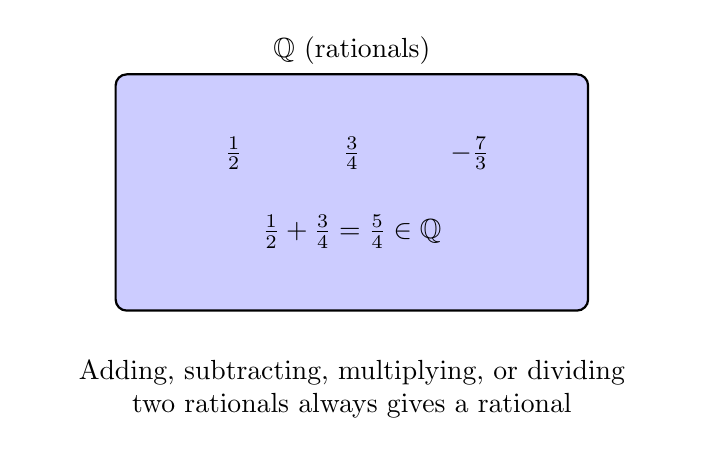
\begin{tikzpicture}[scale=1]
    \draw[thick, rounded corners, fill=blue!20] (-3, -1.5) rectangle (3, 1.5);
    \node at (0, 1.8) {$\mathbb{Q}$ (rationals)};

    \node at (-1.5, 0.5) {$\frac{1}{2}$};
    \node at (0, 0.5) {$\frac{3}{4}$};
    \node at (1.5, 0.5) {$-\frac{7}{3}$};

    \node at (0, -0.5) {$\frac{1}{2} + \frac{3}{4} = \frac{5}{4} \in \mathbb{Q}$};

    \node[text width=8cm, align=center] at (0, -2.5) {Adding, subtracting, multiplying, or dividing\\two rationals always gives a rational};
\end{tikzpicture}
\end{center}

\section{The Proof Strategy: Contradiction}

We use \textbf{proof by contradiction}. Assume the conclusion is false, then derive something impossible.

\begin{center}
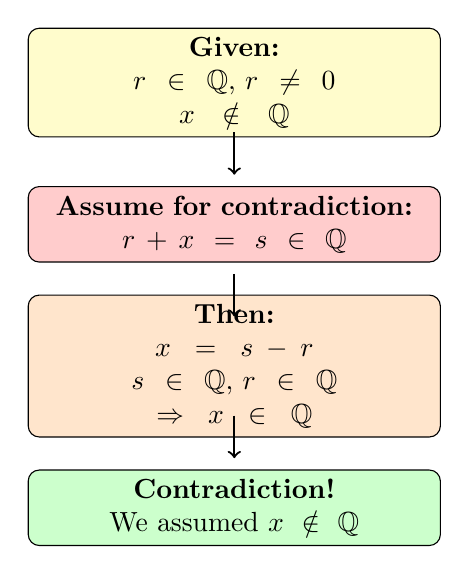
\begin{tikzpicture}[scale=0.9]
    % Setup
    \node[draw, rounded corners, fill=yellow!20, text width=5cm, align=center] at (0, 2) {
        \textbf{Given:}\\
        $r \in \mathbb{Q}$, $r \neq 0$\\
        $x \notin \mathbb{Q}$
    };

    % Assumption
    \node[draw, rounded corners, fill=red!20, text width=5cm, align=center] at (0, 0) {
        \textbf{Assume for contradiction:}\\
        $r + x = s \in \mathbb{Q}$
    };

    % Derivation
    \node[draw, rounded corners, fill=orange!20, text width=5cm, align=center] at (0, -2) {
        \textbf{Then:}\\
        $x = s - r$\\
        $s \in \mathbb{Q}$, $r \in \mathbb{Q}$\\
        $\Rightarrow x \in \mathbb{Q}$
    };

    % Contradiction
    \node[draw, rounded corners, fill=green!20, text width=5cm, align=center] at (0, -4) {
        \textbf{Contradiction!}\\
        We assumed $x \notin \mathbb{Q}$
    };

    \draw[->, thick] (0, 1.3) -- (0, 0.7);
    \draw[->, thick] (0, -0.7) -- (0, -1.3);
    \draw[->, thick] (0, -2.7) -- (0, -3.3);
\end{tikzpicture}
\end{center}

\section{Part 1: $r + x$ is Irrational}

\textbf{Proof:}
\begin{enumerate}
    \item Suppose $r + x = s$ for some $s \in \mathbb{Q}$
    \item Then $x = s - r = s + (-r)$
    \item Since $r \in \mathbb{Q}$, we have $-r \in \mathbb{Q}$
    \item Since $s \in \mathbb{Q}$ and $-r \in \mathbb{Q}$, and $\mathbb{Q}$ is closed under addition: $x = s + (-r) \in \mathbb{Q}$
    \item But we assumed $x$ is irrational — contradiction!
\end{enumerate}

\section{Part 2: $rx$ is Irrational}

\textbf{Proof:}
\begin{enumerate}
    \item Suppose $rx = s$ for some $s \in \mathbb{Q}$
    \item Since $r \neq 0$, the inverse $\frac{1}{r}$ exists
    \item Since $r \in \mathbb{Q}$ and $r \neq 0$, we have $\frac{1}{r} \in \mathbb{Q}$
    \item Then $x = s \cdot \frac{1}{r}$
    \item Since $s \in \mathbb{Q}$ and $\frac{1}{r} \in \mathbb{Q}$, and $\mathbb{Q}$ is closed under multiplication: $x \in \mathbb{Q}$
    \item But we assumed $x$ is irrational — contradiction!
\end{enumerate}

\section{Why $r \neq 0$ Matters for Part 2}

\begin{center}
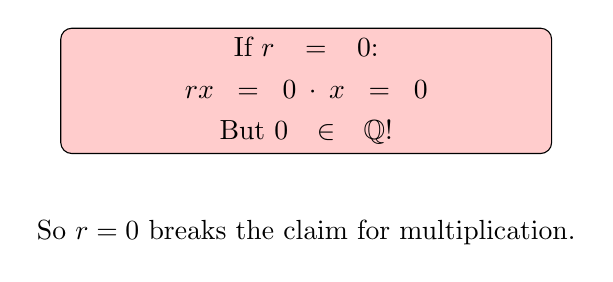
\begin{tikzpicture}[scale=1]
    \node[draw, rounded corners, fill=red!20, text width=6cm, align=center] at (0, 0) {
        If $r = 0$:\\[0.3em]
        $rx = 0 \cdot x = 0$\\[0.3em]
        But $0 \in \mathbb{Q}$!
    };

    \node at (0, -1.8) {So $r = 0$ breaks the claim for multiplication.};
\end{tikzpicture}
\end{center}

\section{Visual Summary: The Number Line}

\begin{center}
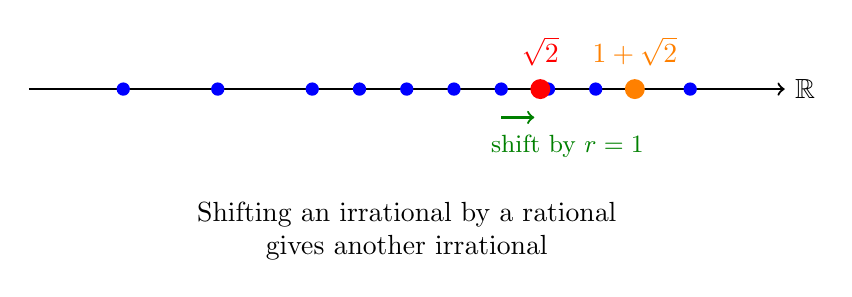
\begin{tikzpicture}[scale=1.2]
    \draw[thick, ->] (-4, 0) -- (4, 0) node[right] {$\mathbb{R}$};

    % Rationals (blue dots)
    \foreach \x in {-3, -2, -1, 0, 1, 2, 3} {
        \fill[blue] (\x, 0) circle (2pt);
    }
    \fill[blue] (-0.5, 0) circle (2pt);
    \fill[blue] (0.5, 0) circle (2pt);
    \fill[blue] (1.5, 0) circle (2pt);

    % An irrational (red)
    \fill[red] (1.414, 0) circle (3pt);
    \node[red] at (1.414, 0.4) {$\sqrt{2}$};

    % r + x
    \fill[orange] (2.414, 0) circle (3pt);
    \node[orange] at (2.414, 0.4) {$1 + \sqrt{2}$};

    \draw[->, thick, green!50!black] (1, -0.3) -- (1.35, -0.3);
    \node[green!50!black] at (1.7, -0.6) {\small shift by $r=1$};

    \node[text width=8cm, align=center] at (0, -1.5) {Shifting an irrational by a rational\\gives another irrational};
\end{tikzpicture}
\end{center}

\section{The Contrapositive View}

The proof by contradiction is equivalent to proving the \textbf{contrapositive}:

\begin{center}
\begin{tabular}{c|c}
\textbf{Original} & \textbf{Contrapositive} \\
\hline
$x$ irrational $\Rightarrow$ $r+x$ irrational & $r+x$ rational $\Rightarrow$ $x$ rational
\end{tabular}
\end{center}

The contrapositive is what we actually showed: if $r + x \in \mathbb{Q}$, then $x = (r+x) - r \in \mathbb{Q}$.

\end{document}
